\documentclass[11pt,a4paper]{article}

% ================= Page Geometry & Typography =================
\usepackage[top=0.88in, bottom=0.88in, left=1in, right=1in, headheight=22pt]{geometry}
\usepackage[T1]{fontenc}
\usepackage[utf8]{inputenc}
\usepackage{lmodern}
\usepackage{microtype}

% ================= Mathematics & Theorem Environments =================
\usepackage{amsmath, amssymb, amsthm}
\usepackage{booktabs}
\usepackage{array}
\usepackage{enumitem}
\usepackage{xcolor}
\usepackage{framed}
\usepackage{tikz}
\usetikzlibrary{arrows.meta, positioning, calc, decorations.pathreplacing}
\usepackage{caption}
\usepackage{fancyhdr}
\usepackage{titlesec}
\usepackage[
  colorlinks=true,
  linkcolor=navyblue,
  citecolor=navyblue,
  urlcolor=navyblue,
  pdftitle={A Combinatorial Proof of Two Tiling Conjectures in OEIS A401673 and Their Rectangular Generalization},
  pdfauthor={Combinatorial Proof Note}
]{hyperref}
\usepackage[capitalize, noabbrev]{cleveref}

% ================= Color Palette =================
\definecolor{navyblue}{HTML}{1B4965}
\definecolor{softblue}{HTML}{EBF3F8}
\definecolor{borderblue}{HTML}{5FA8D3}
\definecolor{warmamber}{HTML}{D97706}
\definecolor{softamber}{HTML}{FEF3C7}
\definecolor{diagteal}{HTML}{0F766E}
\definecolor{softteal}{HTML}{CCFBF1}
\definecolor{slate}{HTML}{475569}
\definecolor{rulegray}{HTML}{CBD5E1}
\definecolor{boxbg}{HTML}{F8FAFC}

% ================= Running Headers & Footers =================
\pagestyle{fancy}
\fancyhf{}
\fancyhead[L]{\footnotesize\color{slate}\textsc{Combinatorial Proof of OEIS A401673 Conjectures}}
\fancyhead[R]{\footnotesize\color{slate}\thepage}
\renewcommand{\headrulewidth}{0.4pt}
\renewcommand{\headrule}{\hbox to\headwidth{\color{rulegray}\leaders\hrule height \headrulewidth\hfill}}
\fancypagestyle{plain}{%
  \fancyhf{}%
  \fancyfoot[C]{\footnotesize\color{slate}\thepage}%
  \renewcommand{\headrulewidth}{0pt}%
}

% ================= Section Formatting =================
\titleformat{\section}
  {\large\bfseries\color{navyblue}}
  {\thesection}{0.75em}{}
\titleformat{\subsection}
  {\normalsize\bfseries\color{navyblue!90!black}}
  {\thesubsection}{0.6em}{}
\titlespacing*{\section}{0pt}{14pt}{6pt}
\titlespacing*{\subsection}{0pt}{10pt}{4pt}

% ================= Theorem Styles =================
\newtheoremstyle{paperthm}
  {8pt}{8pt}{\itshape}{}{\bfseries\color{navyblue}}{.}{0.5em}{}
\newtheoremstyle{paperdef}
  {8pt}{8pt}{\normalfont}{}{\bfseries\color{navyblue}}{.}{0.5em}{}

\theoremstyle{paperthm}
\newtheorem{theorem}{Theorem}
\newtheorem{lemma}{Lemma}
\newtheorem{corollary}{Corollary}
\newtheorem{conjecture}{Conjecture}
\crefname{conjecture}{Conjecture}{Conjectures}
\Crefname{conjecture}{Conjecture}{Conjectures}

\theoremstyle{paperdef}
\newtheorem{remark}{Remark}

\renewcommand{\proofname}{\textbf{\color{navyblue}Proof}}

% Highlighted theorem box (subtle left accent bar)
\newenvironment{accentbox}{%
  \def\FrameCommand{{\color{navyblue}\vrule width 2.2pt}\hspace{10pt}}%
  \MakeFramed{\advance\hsize-\width\FrameRestore}%
}{%
  \endMakeFramed%
}

% Clean boxed result
\newcommand{\resultbox}[1]{%
  \setlength{\fboxsep}{5pt}%
  \fcolorbox{borderblue}{softblue!55}{$\displaystyle #1$}%
}

% List and paragraph defaults
\linespread{1.05}
\setlist{itemsep=2pt, topsep=4pt, parsep=0pt}
\captionsetup{font=small, labelfont={bf, color=navyblue}, margin=8pt}

\begin{document}
\thispagestyle{plain}

% ================= Top-Venue Style Title Block =================
\noindent{\color{navyblue}\rule{\linewidth}{1.6pt}}
\begin{center}
  \vspace{6pt}
  {\LARGE\bfseries\color{navyblue}
    A Combinatorial Proof of Two Tiling Conjectures in\\[3pt]
    OEIS A401673 and Their Rectangular Generalization}\\[10pt]
  {\normalsize\color{slate} Research Note \quad$\cdot$\quad Enumerative Combinatorics}\\[4pt]
  {\small\color{slate} November 25, 2026}
  \vspace{4pt}
\end{center}
\noindent{\color{rulegray}\rule{\linewidth}{0.7pt}}

\vspace{8pt}
\begin{quote}
  \small
  \noindent\textbf{\color{navyblue}Abstract.}
  We resolve two enumerative conjectures recorded in OEIS~A401673 concerning perfect matchings (tilings) of a $2n \times 2n$ chessboard using horizontal, vertical, and diagonal dominoes, where diagonal tiles are permitted to cross within a $2 \times 2$ subgrid. Letting $T(n,k)$ denote the number of valid tilings that contain exactly $2k$ diagonal tiles, we give a self-contained combinatorial proof valid for all $n$ that
  \[
    T(n, n^2) = 1 \qquad\text{and}\qquad T(n, n^2 - 1) = n^2(n+1) \quad (n \ge 1).
  \]
  The proof rests on three elementary structural observations: (i)~a row-parity invariant forcing the total number of horizontal tiles to be even; (ii)~a forced decomposition of any tiling without vertical tiles into $n$ independent $2n \times 2$ vertical strips; and (iii)~a bijection between valid tilings of each vertical strip and one-dimensional sequences of two elementary blocks $H$ and $X$. Using the exact same machinery, we establish a natural generalization to arbitrary even-sided rectangular boards $2m \times 2n$ ($m, n \ge 1$), showing that the all-diagonal tiling remains unique and that the number of tilings with exactly two non-diagonal tiles equals $n\binom{m+1}{2} + m\binom{n+1}{2} = \frac{1}{2}mn(m+n+2)$. Finally, we report an independent backtracking enumeration for $1 \le n \le 7$ that cross-validates the definitions and exact counts.

  \medskip
  \noindent\textbf{\color{navyblue}Keywords:}
  grid tilings, perfect matchings, king's graph, crossing diagonals, enumerative combinatorics, OEIS~A401673.

  \smallskip
  \noindent\textbf{\color{navyblue}MSC 2020:}
  05A15, 05B45, 05C70.
\end{quote}
\vspace{4pt}

% ================= Section 1: Introduction =================
\section{Introduction}

Counting perfect matchings on two-dimensional grid graphs is a classical topic in enumerative combinatorics and statistical physics. While standard domino tilings restrict pairings to orthogonally adjacent cells, a natural variant allows pairs of diagonally adjacent cells---equivalently, perfect matchings of the \emph{king's graph} on a rectangular grid---where two diagonal tiles occupying the same $2 \times 2$ subgrid are permitted to cross~\cite{oeisA239264}.

In November 2026, Dawid Ry\l ko submitted the integer triangle \href{https://oeis.org/A401673}{OEIS~A401673}~\cite{oeisA401673}, which refines the number of such tilings on a $2n \times 2n$ board by the number of diagonal tiles. Specifically, let $T(n,k)$ denote the number of perfect matchings of the $2n \times 2n$ king's graph using exactly $2k$ diagonal edges. The OEIS entry states two closed-form conjectures at the extreme diagonal-rich end of the triangle, verified computationally up to $n \le 10$:
\[
  T(n, n^2) = 1 \qquad\text{and}\qquad T(n, n^2 - 1) = n^2(n+1).
\]

\paragraph{Note on Problem Status and Priority.}
To state the provenance accurately: at the time of lookup, the \href{https://oeis.org/A401673/internal}{OEIS~A401673 internal record} marks both identities as \emph{Conjectures}, and the original author's project page (built November~24, 2026) explicitly describes them as empirical computational observations without proof. No previously published proof was located in our search. While this evidence supports treating the identities as open conjectures, it cannot rule out an unindexed or unpublished proof; formal priority as a first proof should therefore be confirmed by the original author or OEIS editors.

\paragraph{Contributions.}
In this note, we make three concise contributions:
\begin{enumerate}[label=\textbf{(\arabic*)}]
  \item \textbf{Complete proof of both OEIS~A401673 conjectures.} We prove $T(n, n^2) = 1$ for all $n \ge 0$ (\Cref{thm:all-diag}) and $T(n, n^2 - 1) = n^2(n+1)$ for all $n \ge 1$ (\Cref{thm:two-nondiag}) via a transparent, completely elementary reduction from two-dimensional tilings to one-dimensional block sequences.
  \item \textbf{Independent computational cross-check.} We verify the counts for $1 \le n \le 7$ using an unconstrained cell-by-cell backtracking search (\Cref{sec:verification}), confirming exact agreement with both closed forms.
  \item \textbf{Rectangular generalization.} Observing that the structural decomposition does not rely on square symmetry, we extend the proof to arbitrary $2m \times 2n$ boards (\Cref{thm:rectangular}), obtaining the closed form $\frac{1}{2}mn(m+n+2)$ for tilings with exactly two non-diagonal tiles.
\end{enumerate}

% ================= Section 2: Preliminaries =================
\section{Preliminaries and Problem Formulation}
\label{sec:prelim}

Consider a $2n \times 2n$ square grid indexed by $[2n] \times [2n]$, containing $4n^2$ unit cells. A \emph{valid tiling} is a partition of all $4n^2$ cells into $2n^2$ disjoint unordered pairs (\emph{tiles}), where each pair satisfies one of the three adjacency relations summarized in \Cref{tab:tiles}.

\begin{table}[htbp]
  \centering
  \small
  \caption{Admissible tile types on the $2n \times 2n$ chessboard.}
  \label{tab:tiles}
  \begin{tabular}{@{} >{\bfseries}l l @{}}
    \toprule
    Tile Type & Relative Position of the Two Paired Cells \\
    \midrule
    Horizontal & Same row, adjacent columns: $\{(r,c),\,(r,c+1)\}$ \\
    Vertical   & Same column, adjacent rows: $\{(r,c),\,(r+1,c)\}$ \\
    Diagonal   & Adjacent rows and columns (sharing a corner): $\{(r,c),\,(r+1,c\pm 1)\}$ \\
    \bottomrule
  \end{tabular}
\end{table}

Crucially, \textbf{crossing diagonal tiles are permitted}~\cite{oeisA239264}. For instance, a $2 \times 2$ subgrid may be tiled by two crossing diagonal tiles, written schematically as
\[
  \begin{pmatrix} A & B \\ B & A \end{pmatrix},
\]
where identical letters mark the two cells covered by the same tile. \Cref{fig:tiles} illustrates the three tile types together with a crossing diagonal pair.

\begin{figure}[htbp]
  \centering
  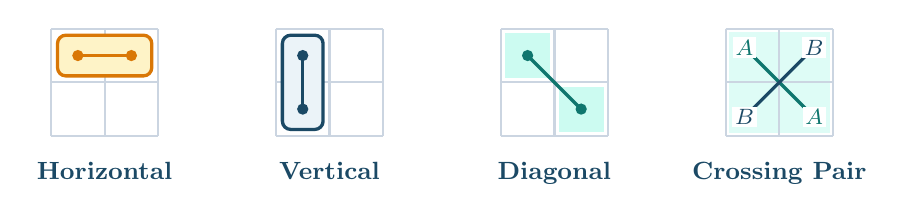
\begin{tikzpicture}[scale=0.68, every node/.style={font=\small}]
    % 1. Horizontal
    \begin{scope}[xshift=0cm]
      \draw[step=1, color=rulegray, thick] (0,0) grid (2,2);
      \fill[softamber, rounded corners=3pt] (0.12,1.12) rectangle (1.88,1.88);
      \draw[warmamber, very thick, rounded corners=3pt] (0.12,1.12) rectangle (1.88,1.88);
      \draw[warmamber, very thick] (0.5,1.5) -- (1.5,1.5);
      \fill[warmamber] (0.5,1.5) circle (3pt) (1.5,1.5) circle (3pt);
      \node[below=6pt, color=navyblue] at (1,0) {\bfseries Horizontal};
    \end{scope}

    % 2. Vertical
    \begin{scope}[xshift=4.2cm]
      \draw[step=1, color=rulegray, thick] (0,0) grid (2,2);
      \fill[softblue, rounded corners=3pt] (0.12,0.12) rectangle (0.88,1.88);
      \draw[navyblue, very thick, rounded corners=3pt] (0.12,0.12) rectangle (0.88,1.88);
      \draw[navyblue, very thick] (0.5,0.5) -- (0.5,1.5);
      \fill[navyblue] (0.5,0.5) circle (3pt) (0.5,1.5) circle (3pt);
      \node[below=6pt, color=navyblue] at (1,0) {\bfseries Vertical};
    \end{scope}

    % 3. Diagonal
    \begin{scope}[xshift=8.4cm]
      \draw[step=1, color=rulegray, thick] (0,0) grid (2,2);
      \fill[softteal] (0.08,1.08) rectangle (0.92,1.92);
      \fill[softteal] (1.08,0.08) rectangle (1.92,0.92);
      \draw[diagteal, very thick] (0.5,1.5) -- (1.5,0.5);
      \fill[diagteal] (0.5,1.5) circle (3pt) (1.5,0.5) circle (3pt);
      \node[below=6pt, color=navyblue] at (1,0) {\bfseries Diagonal};
    \end{scope}

    % 4. Crossing diagonals
    \begin{scope}[xshift=12.6cm]
      \draw[step=1, color=rulegray, thick] (0,0) grid (2,2);
      \fill[softteal!65] (0.06,0.06) rectangle (1.94,1.94);
      \draw[step=1, color=rulegray, thick] (0,0) grid (2,2);
      \draw[diagteal, very thick] (0.45,1.55) -- (1.55,0.45);
      \draw[navyblue, very thick] (0.45,0.45) -- (1.55,1.55);
      \node[fill=white, inner sep=1pt, font=\footnotesize\bfseries, text=diagteal] at (0.35,1.65) {$A$};
      \node[fill=white, inner sep=1pt, font=\footnotesize\bfseries, text=diagteal] at (1.65,0.35) {$A$};
      \node[fill=white, inner sep=1pt, font=\footnotesize\bfseries, text=navyblue] at (1.65,1.65) {$B$};
      \node[fill=white, inner sep=1pt, font=\footnotesize\bfseries, text=navyblue] at (0.35,0.35) {$B$};
      \node[below=6pt, color=navyblue] at (1,0) {\bfseries Crossing Pair};
    \end{scope}
  \end{tikzpicture}
  \caption{The three admissible tile types and a crossing diagonal pairing inside a $2 \times 2$ subgrid.}
  \label{fig:tiles}
\end{figure}

For each integer $k \in \{0, 1, \dots, n^2\}$, define
\[
  T(n,k) \;=\; \bigl|\{\text{valid tilings of the } 2n \times 2n \text{ board containing exactly } 2k \text{ diagonal tiles}\}\bigr|.
\]
The two conjectures posed in OEIS~A401673~\cite{oeisA401673} assert the exact values of the last two entries in row $n$:

\begin{conjecture}[OEIS A401673~\cite{oeisA401673}]
  \label{conj:main}
  For every integer $n \ge 0$, the all-diagonal tiling is unique,
  \[
    T(n, n^2) = 1,
  \]
  and for every integer $n \ge 1$, the number of tilings with exactly two non-diagonal tiles is
  \[
    T(n, n^2 - 1) = n^2(n+1).
  \]
\end{conjecture}

% ================= Section 3: Structural Decomposition =================
\section{Structural Decomposition: From 2D Boards to 1D Words}
\label{sec:structure}

Our proof reduces the two-dimensional matching problem to one-dimensional block arrangements via three elementary lemmas:
\begin{enumerate}[label=(\roman*)]
  \item the total number of horizontal tiles is always even (\Cref{lem:parity});
  \item any tiling devoid of vertical tiles decomposes into $n$ independent adjacent column pairs (\Cref{lem:strips});
  \item each resulting $2n \times 2$ strip is uniquely encoded by a vertical word over two elementary blocks (\Cref{lem:blocks}).
\end{enumerate}

\begin{lemma}[Parity of Horizontal Tiles]
  \label{lem:parity}
  In every valid tiling of a $2n \times 2n$ chessboard, the total number of horizontal tiles is even.
\end{lemma}

\begin{proof}
  Partition the cells of the board by row parity into two sets: $R_{\mathrm{o}}$ consisting of all cells in odd-indexed rows, and $R_{\mathrm{e}}$ consisting of all cells in even-indexed rows. Since there are $n$ odd rows and $n$ even rows, each of length $2n$, we have $|R_{\mathrm{o}}| = |R_{\mathrm{e}}| = 2n^2$.

  Let $h_{\mathrm{o}}$ and $h_{\mathrm{e}}$ denote the numbers of horizontal tiles lying in odd and even rows, respectively, and let $v$ and $d$ denote the total numbers of vertical and diagonal tiles. Every vertical tile and every diagonal tile connects two adjacent rows, hence covers exactly one cell in $R_{\mathrm{o}}$ and one cell in $R_{\mathrm{e}}$. By contrast, each horizontal tile lies within a single row and therefore covers two cells of the same parity class. Double-counting $|R_{\mathrm{o}}|$ and $|R_{\mathrm{e}}|$ yields
  \[
    2n^2 = 2h_{\mathrm{o}} + v + d
    \qquad\text{and}\qquad
    2n^2 = 2h_{\mathrm{e}} + v + d.
  \]
  Subtracting the two identities gives $h_{\mathrm{o}} = h_{\mathrm{e}}$. Thus the total number of horizontal tiles is $h_{\mathrm{o}} + h_{\mathrm{e}} = 2h_{\mathrm{o}}$, which is even.
\end{proof}

\begin{corollary}
  \label{cor:dichotomy}
  In any valid tiling of a $2n \times 2n$ board with exactly two non-diagonal tiles, those two tiles are either \emph{both horizontal} or \emph{both vertical}. A configuration with one horizontal tile and one vertical tile cannot occur.
\end{corollary}

\begin{proof}
  Immediate from \Cref{lem:parity}, since the number of horizontal tiles cannot be $1$.
\end{proof}

\Cref{cor:dichotomy} allows us to analyze the vertical-free (two-horizontal) case first and deduce the two-vertical case by $90^\circ$ rotational symmetry.

\begin{lemma}[Forced Column-Pair Decomposition]
  \label{lem:strips}
  In any valid tiling of a $2n \times 2n$ board containing no vertical tiles, no tile crosses between column $2j$ and column $2j+1$ for any $1 \le j \le n-1$. Consequently, the board decomposes into $n$ mutually independent $2n \times 2$ vertical strips occupying the column pairs
  \[
    (1,2),\quad (3,4),\quad \dots,\quad (2n-1, 2n).
  \]
\end{lemma}

\begin{proof}
  Because no vertical tiles are present, every tile---whether horizontal or diagonal---pairs two cells belonging to adjacent columns. Examine the leftmost column (column~$1$), which contains $2n$ cells. Every cell in column~$1$ must be paired with a distinct cell in column~$2$. Since column~$2$ also contains exactly $2n$ cells, these pairings saturate column~$2$ completely, leaving no cell in column~$2$ available to pair with column~$3$. Removing columns~$1$ and~$2$ and repeating the same argument inductively on the remaining $2n \times (2n-2)$ board yields the stated partition into $n$ independent $2n \times 2$ strips.
\end{proof}

\begin{figure}[htbp]
  \centering
  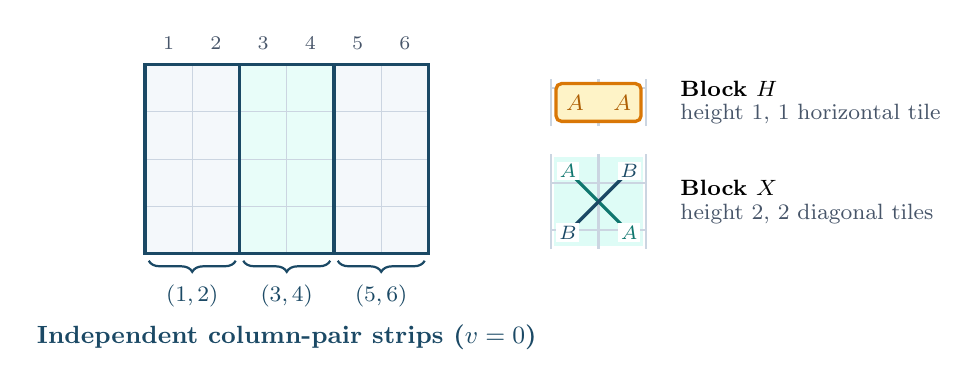
\begin{tikzpicture}[scale=0.60, every node/.style={font=\small}]
    % Left: Column-pair strip decomposition
    \begin{scope}[xshift=0cm]
      \foreach \s/\col in {0/softblue!55, 2/softteal!45, 4/softblue!55} {
        \fill[\col] (\s,0) rectangle (\s+2,4);
      }
      \draw[step=1, color=rulegray, thin] (0,0) grid (6,4);
      \draw[navyblue, very thick] (0,0) rectangle (2,4);
      \draw[navyblue, very thick] (2,0) rectangle (4,4);
      \draw[navyblue, very thick] (4,0) rectangle (6,4);
      \foreach \c in {1,...,6} {
        \node[above=2pt, font=\scriptsize, color=slate] at (\c-0.5, 4) {$\c$};
      }
      \draw[decorate, decoration={brace, amplitude=4pt, mirror}, navyblue, thick]
        (0.08,-0.15) -- (1.92,-0.15) node[midway, below=5pt, font=\footnotesize] {$(1,2)$};
      \draw[decorate, decoration={brace, amplitude=4pt, mirror}, navyblue, thick]
        (2.08,-0.15) -- (3.92,-0.15) node[midway, below=5pt, font=\footnotesize] {$(3,4)$};
      \draw[decorate, decoration={brace, amplitude=4pt, mirror}, navyblue, thick]
        (4.08,-0.15) -- (5.92,-0.15) node[midway, below=5pt, font=\footnotesize] {$(5,6)$};
      \node[below=22pt, color=navyblue, font=\small\bfseries] at (3,0) {Independent column-pair strips ($v=0$)};
    \end{scope}

    % Right: Elementary blocks H and X
    \begin{scope}[xshift=8.6cm, yshift=0.5cm]
      % H block
      \draw[step=1, color=rulegray, thick] (0,2.2) grid (2,3.2);
      \fill[softamber, rounded corners=2pt] (0.1,2.3) rectangle (1.9,3.1);
      \draw[warmamber, very thick, rounded corners=2pt] (0.1,2.3) rectangle (1.9,3.1);
      \node[font=\footnotesize\bfseries, text=warmamber!80!black] at (0.5,2.7) {$A$};
      \node[font=\footnotesize\bfseries, text=warmamber!80!black] at (1.5,2.7) {$A$};
      \node[right=9pt, align=left, font=\footnotesize] at (2,2.7)
        {\textbf{Block $H$}\\[-1pt]\color{slate}height $1$, $1$ horizontal tile};

      % X block
      \draw[step=1, color=rulegray, thick] (0,-0.4) grid (2,1.6);
      \fill[softteal!65] (0.06,-0.34) rectangle (1.94,1.54);
      \draw[step=1, color=rulegray, thick] (0,-0.4) grid (2,1.6);
      \draw[diagteal, very thick] (0.45,1.15) -- (1.55,0.05);
      \draw[navyblue, very thick] (0.45,0.05) -- (1.55,1.15);
      \node[fill=white, inner sep=1pt, font=\scriptsize\bfseries, text=diagteal] at (0.35,1.25) {$A$};
      \node[fill=white, inner sep=1pt, font=\scriptsize\bfseries, text=diagteal] at (1.65,-0.05) {$A$};
      \node[fill=white, inner sep=1pt, font=\scriptsize\bfseries, text=navyblue] at (1.65,1.25) {$B$};
      \node[fill=white, inner sep=1pt, font=\scriptsize\bfseries, text=navyblue] at (0.35,-0.05) {$B$};
      \node[right=9pt, align=left, font=\footnotesize] at (2,0.6)
        {\textbf{Block $X$}\\[-1pt]\color{slate}height $2$, $2$ diagonal tiles};
    \end{scope}
  \end{tikzpicture}
  \caption{Left: forced partition into adjacent column pairs when no vertical tiles are used (\Cref{lem:strips}). Right: the two elementary building blocks $H$ and $X$ governing every vertical strip (\Cref{lem:blocks}).}
  \label{fig:strips-blocks}
\end{figure}

\begin{lemma}[Block Encoding of Vertical Strips]
  \label{lem:blocks}
  Valid vertical-free tilings of a $2n \times 2$ strip are in bijection with top-to-bottom sequences over the alphabet $\{H, X\}$ of total height $2n$, where
  \[
    H = \begin{pmatrix} A & A \end{pmatrix}
    \qquad\text{and}\qquad
    X = \begin{pmatrix} A & B \\ B & A \end{pmatrix}
  \]
  have the dimensions and tile counts listed in \Cref{tab:blocks}. In particular, the number of $H$-blocks in each strip is always even.
\end{lemma}

\begin{proof}
  Inspect the topmost row of a $2n \times 2$ vertical-free strip. Since no vertical tile is permitted, the top-left cell has only two admissible partners:
  \begin{enumerate}[label=\textbf{Case~\arabic*:}, leftmargin=*, align=left]
    \item \emph{It pairs horizontally with the top-right cell.} This forms a single horizontal tile occupying the entire top row, namely the height-$1$ block $H$.
    \item \emph{It pairs diagonally with the cell in row~$2$, column~$2$.} Then the top-right cell cannot pair horizontally (the top-left cell is occupied) and cannot pair vertically ($v = 0$), so it is forced to pair diagonally with the cell in row~$2$, column~$1$. Together, these two tiles completely cover the top two rows as the height-$2$ crossing block $X$.
  \end{enumerate}
  Deleting the top one or two covered rows and iterating inductively establishes the bijection between valid vertical-free tilings of the strip and sequences of $H$- and $X$-blocks of total height $2n$. Finally, if a strip contains $a$ copies of $H$ and $b$ copies of $X$, then
  \[
    a + 2b = 2n,
  \]
  which implies $a = 2(n - b)$ is even.
\end{proof}

\begin{table}[htbp]
  \centering
  \caption{Height and tile-count contributions of the two elementary blocks in a $2n \times 2$ strip.}
  \label{tab:blocks}
  \begin{tabular}{@{} c ccc @{}}
    \toprule
    \textbf{Block} & \textbf{Rows Occupied} & \textbf{Horizontal Tiles} & \textbf{Diagonal Tiles} \\
    \midrule
    $H$ & $1$ & $1$ & $0$ \\
    $X$ & $2$ & $0$ & $2$ \\
    \bottomrule
  \end{tabular}
\end{table}

% ================= Section 4: Main Theorems =================
\section{Proofs of the OEIS A401673 Conjectures}
\label{sec:proofs}

We now prove both parts of \Cref{conj:main}.

\begin{theorem}[Uniqueness of the All-Diagonal Tiling]
  \label{thm:all-diag}
  For every integer $n \ge 0$,
  \[
    \resultbox{T(n, n^2) = 1}.
  \]
\end{theorem}

\begin{proof}
  For $n = 0$, the empty board admits a unique empty tiling. Assume now that $n \ge 1$. A tiling consisting solely of diagonal tiles contains neither vertical nor horizontal tiles. By \Cref{lem:strips}, the board decomposes into $n$ independent $2n \times 2$ vertical strips. By \Cref{lem:blocks}, each strip must be tiled exclusively with $X$-blocks (since $H$-blocks introduce horizontal tiles), forcing the unique word $X^n = \underbrace{XX\cdots X}_{n}$ in every strip. Because all $n$ strips are uniquely determined, $T(n, n^2) = 1$.
\end{proof}

\begin{theorem}[Exact Count for Two Non-Diagonal Tiles]
  \label{thm:two-nondiag}
  For every integer $n \ge 1$,
  \[
    \resultbox{T(n, n^2 - 1) = n^2(n+1)}.
  \]
\end{theorem}

\begin{proof}
  By \Cref{cor:dichotomy}, any valid tiling of the $2n \times 2n$ board with exactly two non-diagonal tiles falls into one of two disjoint classes: either both non-diagonal tiles are horizontal, or both are vertical. We count the two-horizontal class first.

  \paragraph{Step 1: Concentration within a single strip.}
  Since no vertical tiles occur, \Cref{lem:strips} partitions the board into $n$ independent $2n \times 2$ strips. By \Cref{lem:blocks}, each strip contains an \emph{even} number of $H$-blocks. Because the entire board has exactly two $H$-blocks in total, both $H$-blocks must reside in the same strip, while the remaining $n-1$ strips contain zero $H$-blocks. There are $n$ ways to choose the unique strip containing the two horizontal tiles.

  \paragraph{Step 2: Intra-strip arrangement count.}
  In the chosen $2n \times 2$ strip, the two $H$-blocks occupy $2$ rows and the remaining $2n - 2$ rows are covered by $n - 1$ copies of $X$. By \Cref{lem:blocks}, the valid tilings of this strip are in bijection with all words containing two $H$'s and $n-1$ $X$'s---a total of $n+1$ blocks, among which choosing the two positions of $H$ yields
  \[
    \binom{n+1}{2}
  \]
  distinct arrangements. (For example, when $n = 2$, the $4 \times 2$ strip admits $\binom{3}{2} = 3$ words: $HHX$, $HXH$, and $XHH$; see \Cref{fig:n2-words}.) Each of the other $n-1$ strips contains no $H$-blocks and is therefore uniquely tiled as $X^n$. Consequently, the number of tilings with exactly two horizontal tiles is
  \[
    n\binom{n+1}{2}.
  \]

  \begin{figure}[htbp]
    \centering
    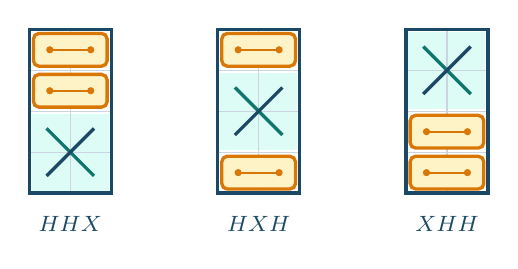
\begin{tikzpicture}[scale=0.52, every node/.style={font=\footnotesize}]
      \newcommand{\drawH}[2]{%
        \fill[softamber, rounded corners=2pt] (#1+0.1,#2+0.1) rectangle (#1+1.9,#2+0.9);
        \draw[warmamber, very thick, rounded corners=2pt] (#1+0.1,#2+0.1) rectangle (#1+1.9,#2+0.9);
        \draw[warmamber, thick] (#1+0.5,#2+0.5) -- (#1+1.5,#2+0.5);
        \fill[warmamber] (#1+0.5,#2+0.5) circle (2.5pt) (#1+1.5,#2+0.5) circle (2.5pt);
      }
      \newcommand{\drawX}[2]{%
        \fill[softteal!65] (#1+0.06,#2+0.06) rectangle (#1+1.94,#2+1.94);
        \draw[step=1, color=rulegray, thin] (#1,#2) grid (#1+2,#2+2);
        \draw[diagteal, very thick] (#1+0.42,#2+1.58) -- (#1+1.58,#2+0.42);
        \draw[navyblue, very thick] (#1+0.42,#2+0.42) -- (#1+1.58,#2+1.58);
      }

      \begin{scope}[xshift=0cm]
        \draw[step=1, color=rulegray, thin] (0,0) grid (2,4);
        \drawH{0}{3} \drawH{0}{2} \drawX{0}{0}
        \draw[navyblue, very thick] (0,0) rectangle (2,4);
        \node[below=5pt, color=navyblue] at (1,0) {$HHX$};
      \end{scope}

      \begin{scope}[xshift=4.6cm]
        \draw[step=1, color=rulegray, thin] (0,0) grid (2,4);
        \drawH{0}{3} \drawX{0}{1} \drawH{0}{0}
        \draw[navyblue, very thick] (0,0) rectangle (2,4);
        \node[below=5pt, color=navyblue] at (1,0) {$HXH$};
      \end{scope}

      \begin{scope}[xshift=9.2cm]
        \draw[step=1, color=rulegray, thin] (0,0) grid (2,4);
        \drawX{0}{2} \drawH{0}{1} \drawH{0}{0}
        \draw[navyblue, very thick] (0,0) rectangle (2,4);
        \node[below=5pt, color=navyblue] at (1,0) {$XHH$};
      \end{scope}
    \end{tikzpicture}
    \caption{All $\binom{3}{2} = 3$ vertical-free tilings of a $4 \times 2$ strip ($n=2$) containing two $H$-blocks and one $X$-block.}
    \label{fig:n2-words}
  \end{figure}

  \paragraph{Step 3: Rotational symmetry.}
  Rotating the $2n \times 2n$ board by $90^\circ$ preserves diagonal tiles while interchanging horizontal and vertical tiles, establishing a bijection between tilings with two horizontal tiles and tilings with two vertical tiles. Since the two classes are disjoint and exhaustive, we conclude that
  \[
    T(n, n^2 - 1)
    \;=\; 2n\binom{n+1}{2}
    \;=\; 2n \cdot \frac{n(n+1)}{2}
    \;=\; \resultbox{n^2(n+1)}. \qedhere
  \]
\end{proof}

% ================= Section 5: Verification =================
\section{Independent Computational Verification}
\label{sec:verification}

To cross-check the problem formulation and exact counts independently of the structural lemmas above, an exhaustive cell-by-cell backtracking program was executed to enumerate perfect matchings of the $2n \times 2n$ king's graph. At each recursion step, the search selects the first uncovered cell and branches over all admissible horizontal, vertical, and diagonal pairings, pruning branches once the number of non-diagonal tiles exceeds two; none of the structural decomposition or closed-form formulas are encoded in the solver.

\begin{table}[htbp]
  \centering
  \small
  \setlength{\tabcolsep}{6pt}
  \caption{Exact counts from independent backtracking enumeration versus the closed-form formulas for $1 \le n \le 7$.}
  \label{tab:verification}
  \begin{tabular}{@{} c c c c c @{}}
    \toprule
    $n$ & \textbf{Board Size} & \textbf{All-Diagonal} $T(n, n^2)$ & \textbf{Two Non-Diagonal} $T(n, n^2 - 1)$ & \textbf{Formula} $n^2(n+1)$ \\
    \midrule
    $1$ & $2 \times 2$   & $1$ & $2$   & $2$   \\
    $2$ & $4 \times 4$   & $1$ & $12$  & $12$  \\
    $3$ & $6 \times 6$   & $1$ & $36$  & $36$  \\
    $4$ & $8 \times 8$   & $1$ & $80$  & $80$  \\
    $5$ & $10 \times 10$ & $1$ & $150$ & $150$ \\
    $6$ & $12 \times 12$ & $1$ & $252$ & $252$ \\
    $7$ & $14 \times 14$ & $1$ & $392$ & $392$ \\
    \bottomrule
  \end{tabular}
\end{table}

\Cref{tab:verification} confirms exact agreement across all tested sizes $1 \le n \le 7$. This computation serves solely as a sanity check on definitions and small-$n$ counts; validity for general $n$ is established unconditionally by \Cref{thm:all-diag,thm:two-nondiag}.

% ================= Section 6: Rectangular Generalization =================
\section{Generalization to Rectangular \texorpdfstring{$2m \times 2n$}{2m x 2n} Boards}
\label{sec:rectangular}

Notably, none of the structural ingredients in \Cref{sec:structure} require the board to be square. Replacing the $2n \times 2n$ grid by an arbitrary even-sided rectangular board with $2m$ rows and $2n$ columns ($m, n \ge 1$) yields an immediate generalization.

\begin{accentbox}
  \begin{theorem}[Rectangular Board Generalization]
    \label{thm:rectangular}
    On a $2m \times 2n$ chessboard ($m, n \ge 1$) permitting crossing diagonal tiles, the all-diagonal tiling is unique, and the number of valid tilings with exactly two non-diagonal tiles is
    \[
      \resultbox{
        n\binom{m+1}{2} + m\binom{n+1}{2}
        \;=\;
        \frac{mn(m + n + 2)}{2}.
      }
    \]
  \end{theorem}
\end{accentbox}

\begin{proof}
  Each of the three structural lemmas carries over verbatim to the $2m \times 2n$ grid:
  \begin{itemize}
    \item \emph{Row- and column-parity invariants.} Partitioning cells by row parity yields two sets of size $2mn$, so $2mn = 2h_{\mathrm{o}} + v + d = 2h_{\mathrm{e}} + v + d$, forcing the number of horizontal tiles to be even. By transposition (column parity), the number of vertical tiles is also even. Hence any tiling with exactly two non-diagonal tiles has either two horizontal tiles or two vertical tiles.
    \item \emph{All-diagonal and two-horizontal cases.} When $v = 0$, the board decomposes into $n$ independent vertical strips of size $2m \times 2$, each uniquely encoded as a sequence of $H$- and $X$-blocks with $a + 2b = 2m$, so each strip holds an even number of $H$-blocks. When no non-diagonal tiles occur, every strip is uniquely $X^m$, giving a unique all-diagonal tiling. When two horizontal tiles occur, both must lie in a single strip ($n$ choices), inside which two $H$-blocks and $m-1$ $X$-blocks can be arranged in $\binom{m+1}{2}$ ways while the remaining $n-1$ strips are uniquely $X^m$. This yields $n\binom{m+1}{2}$ tilings.
    \item \emph{Two-vertical case via transposition.} Transposing the $2m \times 2n$ board to a $2n \times 2m$ board bijectively maps two-vertical tilings onto two-horizontal tilings of the transposed board, contributing $m\binom{n+1}{2}$ tilings.
  \end{itemize}
  Summing the two disjoint classes gives
  \[
    n\binom{m+1}{2} + m\binom{n+1}{2}
    = \frac{nm(m+1) + mn(n+1)}{2}
    = \frac{mn(m + n + 2)}{2}. \qedhere
  \]
\end{proof}

Setting $m = n$ in \Cref{thm:rectangular} immediately yields $\frac{1}{2}n^2(2n+2) = n^2(n+1)$, recovering \Cref{thm:two-nondiag}.

% ================= Section 7: Concluding Remarks =================
\section{Concluding Remarks}

We have presented a self-contained, elementary combinatorial proof of both conjectures in OEIS~A401673 together with their exact extension to $2m \times 2n$ rectangular boards. The key mechanism is that prohibiting vertical tiles collapses the two-dimensional matching geometry into independent width-$2$ strips governed by a binary block alphabet $\{H, X\}$, and the row-parity invariant guarantees that a total budget of two non-diagonal tiles cannot be split between horizontal and vertical orientations. An interesting direction for future work is the enumeration of $T(n, n^2 - r)$ for $r \ge 2$, where simultaneous horizontal and vertical tiles ($h \ge 2$ and $v \ge 2$) become permissible and couple adjacent column-pair strips.

Every mathematical step in this note is completely self-contained and verifiable line by line; as noted in the introduction, establishing formal priority as the first public proof remains subject to confirmation by the original author or OEIS editors.

% ================= References =================
\begin{thebibliography}{9}

\bibitem{oeisA401673}
D.~Ry\l ko,
\emph{Sequence A401673},
in The On-Line Encyclopedia of Integer Sequences (OEIS),
submitted November~1, 2026.
Available at \url{https://oeis.org/A401673} (internal record: \url{https://oeis.org/A401673/internal}).

\bibitem{oeisA239264}
OEIS Foundation Inc.,
\emph{Sequence A239264 (Number of matchings/tilings of grids with crossing diagonal pairs)},
in The On-Line Encyclopedia of Integer Sequences (OEIS).
Available at \url{https://oeis.org/A239264/internal}.

\end{thebibliography}

\end{document}
